\documentclass{sig-alternate-05-2015}
\usepackage{float}
\usepackage{hyperref}
\usepackage{subcaption}
\usepackage{booktabs}
\usepackage{algorithmic}

\begin{document}
\title{Transferring Big Data in Bioinformatics}

\numberofauthors{1}
\author{
\alignauthor Andrew van Rooyen\\
\affaddr{University of Cape Town}\\
\email{Andrew.vanRooyen@alumni.uct.ac.za}
}

\date{30 August 2015}

\toappear{
This paper and associated code is available at \url{https://github.com/wraithy/bigbinf}\\
The OpenSSH-Portable installation used for HPN-SSH was compiled from \url{https://github.com/rapier1/openssh-portable}\\
The large hg38.fa.align.gz dataset used is available at \url{http://hgdownload.cse.ucsc.edu/goldenPath/hg38/bigZips/}\\
For more information, please see \url{pubs.cs.uct.ac.za}
}

\maketitle
\begin{abstract}
Data transfer remains a necessity for research in Bioinformatics, and alternate solutions like cloud computing have not removed the need completely. When transferring large files, there are many transfer protocols to choose from. In this paper, a lightweight testbed is described and used to test SCP, FTP, HPN-SCP and GridFTP between the Universities of Cape Town and the Western Cape.

A comparison of GridFTP's `UDT' mode and it's default mode is also done using the same testbed.

Investigation is done into how the transfer protocols operate on a congested network. Speed and data efficiency are then compared on a stable network to determine if any one protocol is significantly better than the rest.
\end{abstract}

\section{Introduction}
Next generation sequencing has resulted in a massive increase in the size of bioinformatics datasets, which can be tens of gigabytes in size~\cite{deorowicz2011compression}. Sequencing technologies like SOLiD provide much higher data output at a cheaper cost~\cite{shendure2008next}, which creates challenges in data storage, transfer and access. In fact, the cost of storing a byte has been higher than sequencing a base pair since before 2010~\cite{baker2010next}.

Generally, sequence data is stored in a data warehouse. Storing this information for long periods of time requires the data to be structured efficiently in order to save space and to allow it to be transferred efficiently.

There are a plethora of sequence file formats whose efficiency depends on the kind of data stored. Two of the most popular are FASTQ, which stores aggregated reads along with the quality of each DNA base pair~\cite{cock2010sanger}, and BAM, the binary, compressed version of the Sequence Alignment Map (SAM) format~\cite{SAMspec}.

Researchers often require access to the data warehouses to transfer the sequences they need. Luckily, these locations are often connected by massive data pipes like National Research and Education Networks (NREN's). For example, South African universities are connected by the South African National Research Network~\cite{sanren} which runs at 10Gbps. Unfortunately, standard transfer protocols like FTP and SSH were not designed for use on high-throughput networks, and alternate protocols must be used to avoid bottlenecks.

Some proprietary transfer protocols are widely used in practice \emdash for example, the \textit{fasp} protocol by the US based company AsperaSoft. Based on UDP, this protocol eliminates the latency issues seen with TCP, and provides transfer bandwidth of up to 10 gigabits per second~\cite{fan2010petabytes}.

There have been some attempts to avoid data transfer altogether. This means processing data remotely, and there has been an explorative push towards cloud solutions from companies such as Amazon and Google~\cite{baker2010next}. Unfortunately, even though cloud data centres have plenty of cheap storage, the transfer bottleneck remains as researchers must still upload their raw data to the cloud data centres every time they run a new experiment. Some researchers have even resorted to mailing hard drives~\cite{baker2010next}.

There are also security, privacy and ethical concerns with outsourcing processing power to other companies, as sequenced DNA data is often highly sensitive information~\cite{marx2013biology}.

Although it would be ideal for researchers if this reliance on data transfer was removed, the current solutions do not provide good enough answers at every scale. Therefore, transferring big data is still a necessary evil for the time being.

In situations where data \textit{must} be transferred, it stands to reason that the transfer should happen in the most efficient way.

In this work, we construct a testbed which can be deployed on a network to test various transfer protocols. The testbed is outlined, and then used to test SCP, FTP, GridFTP and HPN-SCP. These are the most popular protocols for file transfer in the field, perhaps with the exception of AsperaSoft's \textit{fasp}, which is non-free. 

In order to test the protocols in a relevant environment, the tests are run between the University of Cape Town (UCT) and the University of the Western Cape (UWC) which are connected via SANReN.

\section{Methods}
A testbed is created to measure speed, data efficiency and packet size of specific transfer protocols. Transfers are run and information about them is captured and saved. These logs are then analysed and displayed visually. The testbed does not try to come up with the `best transfer protocol', but rather presents the information relevant to the specific environment so that the user can make decisions.

\subsection{Testbed Design}
The testbed has been designed to be simple, modular and extensible. A simple Python system is sufficient, because almost all of the work transferring and logging the data is done by external programs. The testbed simply acts as a mediator between them.

The data dump format is a simple json template, and can be parsed by the separate analysis code.

The protocols to be tested are specified in a config file, and have no imposed limits. As long as the correct binaries are installed on the machine, a user could test any transfer program as long as they know the command line arguments.

The testbed itself is designed to have minimal dependencies, while the optional analysis notebook makes heavy use of Python data science packages.

The logging mechanism makes use of the `tcpdump' program~\cite{tcpdump}, which comes with most Unix-like systems. As depicted in Figure~\ref{fig:copy_example}, it watches a network interface (e.g.\ eth0) and logs information about packets which pass through. The program is run while each transfer is in progress, and the output is filtered to include only packets sent between Host 1 and Host 2. This output is used as the raw data for analysis.

The Python program for running the file transfers has been written to accept: the name of the network interface, the remote hostname (Host 2), the path of the file on Host 2, and a local path to copy the file to.
It then resolves the IPs of each host, and for each protocol, runs a transfer in isolation. 

\begin{figure}[t]
\centering
	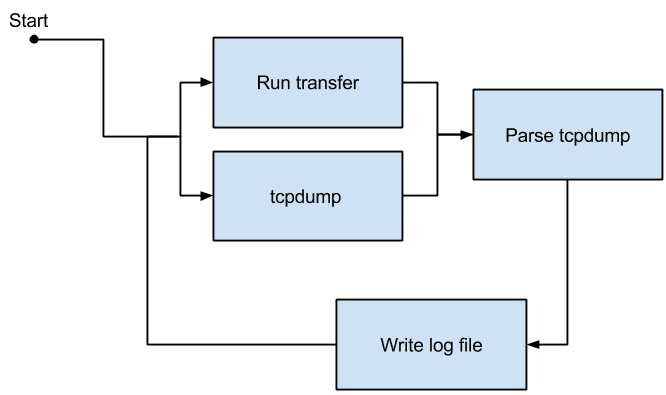
\includegraphics[width=.8\linewidth]{img/loop}
\caption{The sequence of actions performed by the testbed. This is repeated once for each protocol.\label{fig:testbed_sequence}}
\end{figure}

As shown in Figure~\ref{fig:testbed_sequence}, it spawns a tcpdump subprocess which runs for precisely as long as the copy runs. The tcpdump program is started with filters, so that only traffic between the two hosts is captured. It then saves the output in a file.

This allows for a controlled environment, because tcpdump only captures while the copy is running, no other packets are included in the logs. Also, the copies are run programmatically and consecutively. Successive copies are not started until both the tcpdump and protocol processes have been closed, and the log file has been written. This means that they are all run in an identical (within reason) environment, but at the same time do not interfere with each other.

This test process is run multiple times for statistical reasons, generating multiple log files.

A Jupyter notebook~\cite{jupyter} is provided to read in the dump files. This information can be aggregated, and then used to calculate metrics and display graphs. These include plots which are computed by looking at the time of each packet, and the size of its payload.

The testbed was simultaneously tested between various locations. During early stages, tests were run between lab computers at UCT. These were naturally on the same LAN. This meant that there was no interference or issues with stability, but the network was capped at 100Mbit/s. Because all the protocols could easily reach this speed, the results from different tests didn't reveal much.

The testbed was then deployed between a home network in Cape Town, and a Virtual Private Server in Amsterdam. The speed was again capped, but this enabled testing under unstable conditions, and the testbed had to be made more robust.

\subsection{Test Case between UCT and UWC}
The testbed is deployed between two hosts to test that the binaries for each transfer protocol are set up correctly (both on the client and server). Once ready, a full set of tests is run between them.

\begin{figure}[t]
\centering
	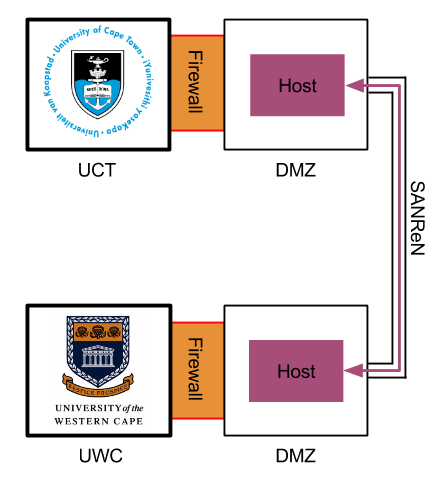
\includegraphics[width=.6\linewidth]{img/route.png}
\caption{The hosts in their environment.\label{fig:route}}
\end{figure}

The hosts are virtual machines running at the South African National Bioinformatics Institute (UWC) and the Science DMZ (UCT). Both locations are close to the SANReN link, and outside institutional firewalls as depicted in Figure~\ref{fig:route}. This means that throttling is avoided, and ensures a speed of up to 1Gbps.

Four different protocols were chosen to be tested. Two of the most widely used are FTP and SCP, and each of these has a more recent successor (GridFTP and HPN-SCP respectively).

Transfers using each of the four protocols are run while the network traffic is logged.

The testing environment is kept as stable as possible during tests, and multiple tests are run at different times of the day.

\begin{figure}[t]
\centering
	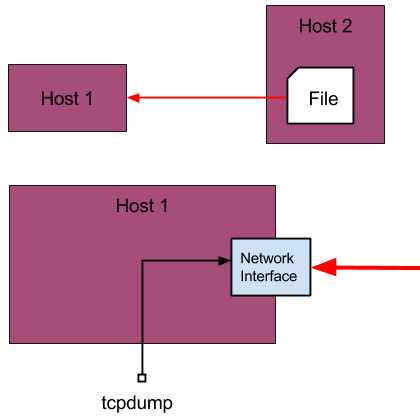
\includegraphics[width=.6\linewidth]{img/transfer_example.png}
\caption{Host 1 copying a file and capturing packets.\label{fig:copy_example}}
\end{figure}
For each transfer, a copy is initiated from Host 1. A file from Host 2 is transferred to Host 1 using the particular protocol (see Figure~\ref{fig:copy_example}).

The tests are run with 6 files. These are one small 5MiB file, and five files between 0.5GiB and 2.4GiB in 0.5GiB increments. These were all generated by reading chunks of a 2.4 GB gzipped sequence alignment file. Even though the protocols are agnostic of file format (they treat everything as binary), the sequence alignment file is a typical dataset that researchers would need to transfer.

\subsection{Protocols}
The OpenSSH~\cite{openssh} implementations of FTP (sftp) and SSH (scp) are tested. High Performance SSH (HPN-SSH) is a set of patches to OpenSSH which removes bottlenecks~\cite{rapier2008high}. The scp binary from a patched, portable version of OpenSSH is tested for HPN\@. This is installed alongside the original so that both binaries are available.

The `lite' version of GridFTP~\cite{allcock2005globus} is used. This means that authentication is done via ssh as opposed a previously-configured certificate authority. This makes no difference to the file transfer itself, but it prevents unnecessary configuration of the testbed which can be quite complex in the case of `full' GridFTP~\cite{gridftplite}.

GridFTP supports data `striping', which allows a transfer to be split across multiple hosts, potentially combining their bandwidths. This feature is not used, because the number of available nodes can vary greatly between configurations, and it would make comparisons with single-stream transfers unrealistic.

GridFTP also provides two modes of general operation. The default mode operates on top of the TCP stack, but there is a newer `UDT' mode which is based on UDP\@. This mode aims to overcome congestion control bottlenecks found in TCP\@. Although Bresnahan et al.\ found that the UDT mode outperformed the TCP mode~\cite{bresnahan2009udt}, both modes are still tested. Note that despite it's name, the tcpdump program will capture UDP packets.

\subsection{Data collection}
Results were collected by running the testbed at 13h00 and 3h00 each day, for a period of two weeks. For some of the tests, all the collected data (including information about each packet) was stored to disk. Because this is very space intensive (a single test run could generate multiple gigabytes of dump files), most of the tests only stored their aggregated data. 

The measures were chosen by practicality. For example, behind the scenes information like window sizes is not collected, because the biggest concern for users is speed and size.

The tests were scheduled using the `cron' daemon. Each job would call a script that looks like the following.

\begin{algorithm}
\caption{Script to run one round of tests.}
	\begin{algorithmic}
		\STATE SIZES = 5M 512M 1G 1\_5G 2G 2\_4G
		\FOR{ROUND in \{0..4\}}
		\FOR{S in SIZES}
		\STATE Run transfer for S using testbed
		\ENDFOR
		\ENDFOR
	\end{algorithmic}
\label{alg:script}
\end{algorithm}

\section{Results}

Even though the network could theoretically support up to 1Gbit/s, the speeds achieved throughout these tests were around 200Mbit/s. Although this is not as high as hoped, it is still a massive speedup over conventional South African networks, and these speeds are still typical to the use case in the field.

\subsection{Network stability}
Although each transfer in one test runs in the same environment, the time that tests are run can influence the results if the network is busier at certain times of the day.

\begin{figure}
\centering
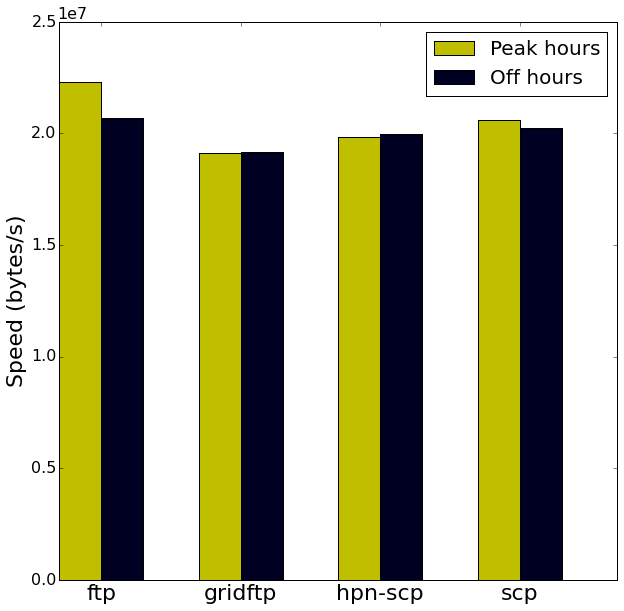
\includegraphics[width=.8\linewidth]{img/peak.png}
\caption{Aggregated comparison of speed during peak and off hours.}
\label{fig:peak}
\end{figure}

\begin{table}
\centering
	\begin{tabular}{lr}
	\toprule
	Protocol &  p-value \\
	\midrule
	ftp         &      0.4 \\
	scp         &      0.5 \\
	hpn-scp     &      0.7 \\
	gridftp     &      0.4 \\
	gridftp-udt &      0.9 \\
	\bottomrule
	\end{tabular}
\caption{p-values for a T-Test between the two sets, with null hypothesis that the speeds are the same.}
\label{tab:pval}
\end{table}

Figure~\ref{fig:peak} is a conventional summary of the speed at various times in the day. "Peak hours" were considered to be between 11h00 and 15h00, and all tests were either in this time frame (peak) or not (off hours). Interestingly, TCP based protocols tend to be slightly faster than GridFTP-UDT during peak hours, while the opposite is true during off hours. However, even though some might appear faster, a t-test between each set of subgroups reveals that the differences are not statistically significant. The p-values from this test can be seen in Table~\ref{tab:pval}, and their values are clearly quite large (meaning that we cannot reject the null hypothesis).

\begin{figure*}
\centering
	\begin{subfigure}{.4\linewidth}
	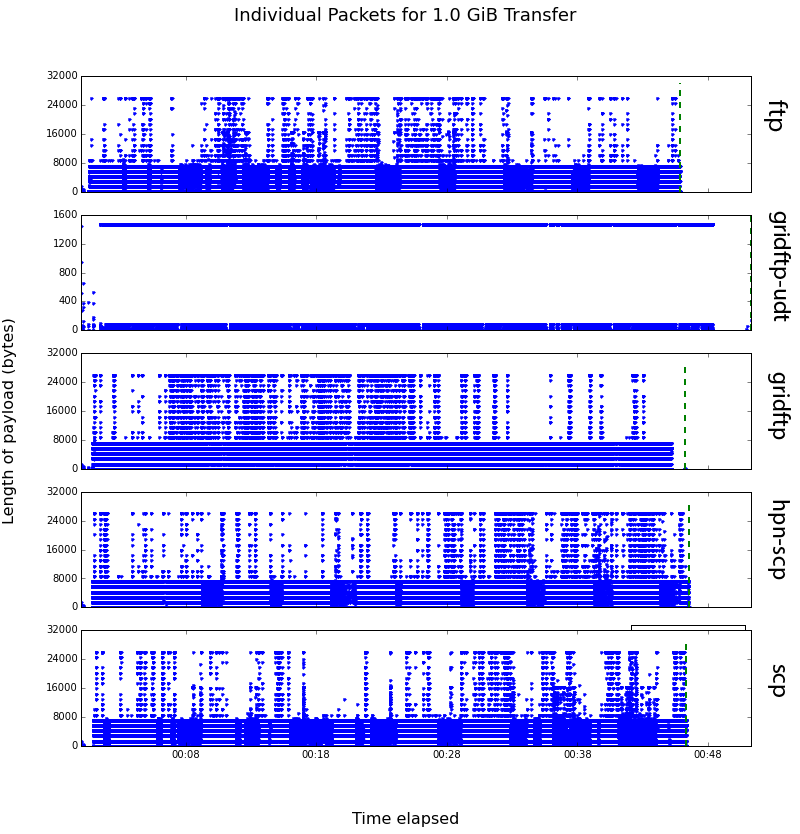
\includegraphics[width=\linewidth]{img/packets/good.png}
	\caption{Stable network}
	\label{fig:good_transfer}
	\end{subfigure}
	\begin{subfigure}{.4\linewidth}
	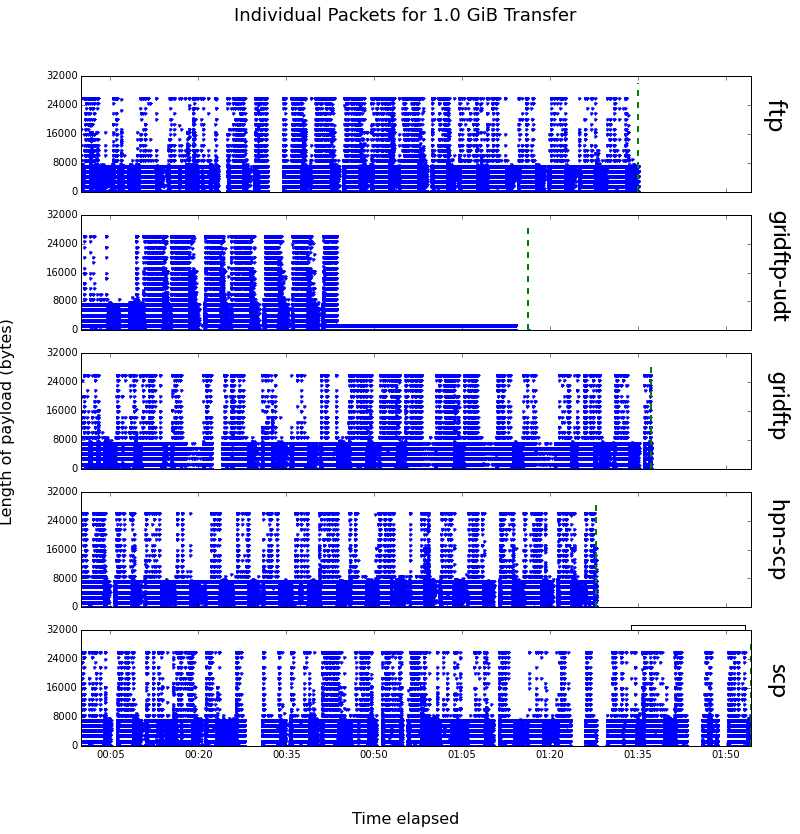
\includegraphics[width=\linewidth]{img/packets/bad.png}
	\caption{Unstable network}
	\label{fig:bad_transfer}
	\end{subfigure}
\caption{A graphical fingerprint of each transfer run under two network conditions. Each point on the graph represents a packet.}
\label{fig:packets}
\end{figure*}

While the stability of the network at each time affects the speed of the transfers, but it is sometimes useful to look other, more subtle effects as well. 

Figure~\ref{fig:packets} represents  one complete transfer for each transfer protocol, for one file size (five rotations of Figure~\ref{fig:testbed_sequence}). This test is shown as a time series, where each point on the plot represents a packet. Both incoming and outgoing packets are plotted, and the height of each packet represents the size of it's payload. In this case, there was a confirmed instability at the specific date and time that Figure~\ref{fig:bad_transfer} was captured. Note that transfers in Figure~\ref{fig:good_transfer} take about 45 seconds, while in Figure~\ref{fig:bad_transfer} they take over 1.5 minutes.

Firstly, comparing Figure~\ref{fig:good_transfer} and Figure~\ref{fig:bad_transfer} confirms that transfers on a busy network do take longer. Secondly, the comparison shows how each transfer protocol handles the congestion. The fingerprints for the TCP based protocols are very similar, but close inspection shows that the unstable transfers are more clustered. The stable transfers are sparsely populated but somewhat consistent, while the unstable transfers have distinct `bands' with densely packed columns separated by thinner gaps with no packets. A likely explanation for this is that a router on one of the hops (most likely the first hop) was congested and had to buffer packets until space was made. This is a typical side effect of congestion on packet switching networks.

The UDP-based UDT mode of GridFTP changes in a more obvious way. Note that the axis limit doubles from the stable to unstable plot. This mode tries to match it's packet sizes to the network MTU (Maximum Transmission Unit) for efficiency. The MTU for the ethernet interface on the test machine was 1500, and Figure~\ref{fig:good_transfer} is an example of the transfer operating in ideal conditions, consistently achieving this size. However, it is clear from Figure~\ref{fig:bad_transfer} that the first half of the transfer was congested, and a bigger payload is forced into each packet. This is only one of the factors that influence transfer speed, but it clearly does have a negative impact.

Because the differences in Figure~\ref{fig:peak} are not statistically significant, all tests are used for the following analysis.

\subsection{Speed and Data Efficiency}

\begin{figure}[h]
\centering
	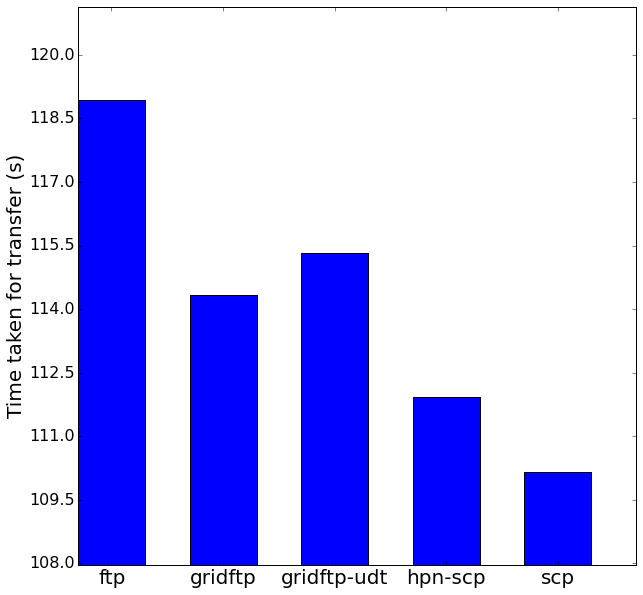
\includegraphics[width=.8\linewidth]{img/time.png}
\caption{Total average time to transfer a 2.4GiB file. Smaller values are better.}
\label{fig:time}
\end{figure}

Figure~\ref{fig:time} is a very simple plot of the average time taken to transfer the largest file. This by no means allows one to see the full picture, but it is useful if you want to find out which protocol will move your data in the shortest time. The SCP and HPN-SCP are the fastest, and both GridFTP modes finish roughly 5 seconds later. FTP is the slowest, taking 8.7 more seconds, which is 7.9\% more time than SCP.

At this stage is is useful to note that while GridFTP has improved upon FTP, the HPN patches to SCP have not sped up the transfer on this specific network configuration. Also, the improvement of GridFTP only holds true for this specific file size. A complete comparison for all file sizes can be found in Figure~\ref{fig:per_fs_speed}.

\begin{figure*}[t]
\centering
	\begin{subfigure}{.3\linewidth}
	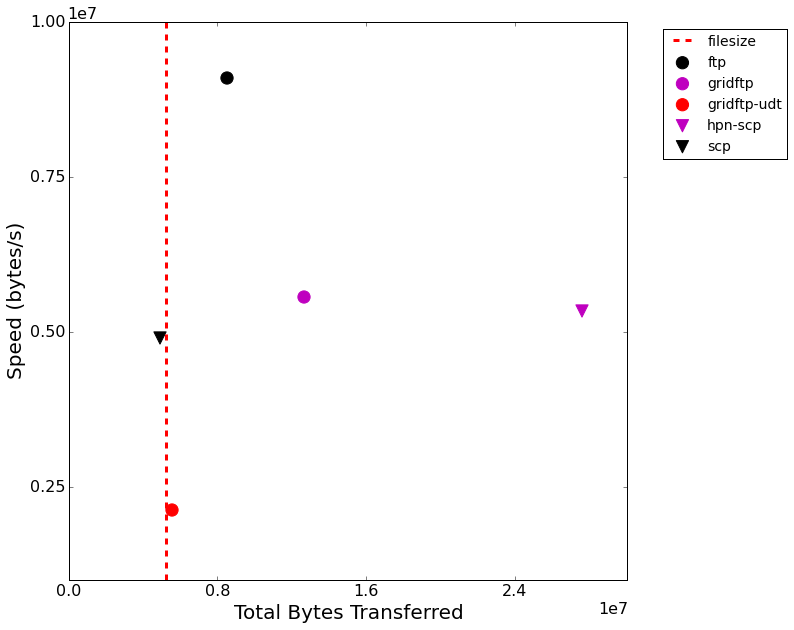
\includegraphics[width=\linewidth]{img/speed_bytes/5M.png}
	\caption{5 Megabytes}
	\label{speed_bytes_5M}
	\end{subfigure}
	\begin{subfigure}{.3\linewidth}
	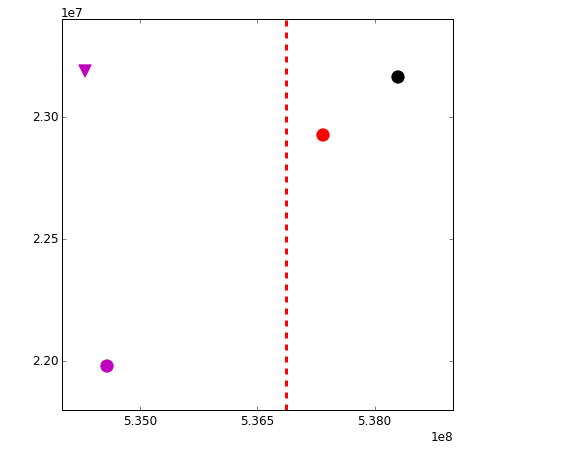
\includegraphics[width=\linewidth]{img/speed_bytes/512M.png}
	\caption{0.5 Gigabytes}
	\label{speed_bytes_512M}
	\end{subfigure}
	\begin{subfigure}{.3\linewidth}
	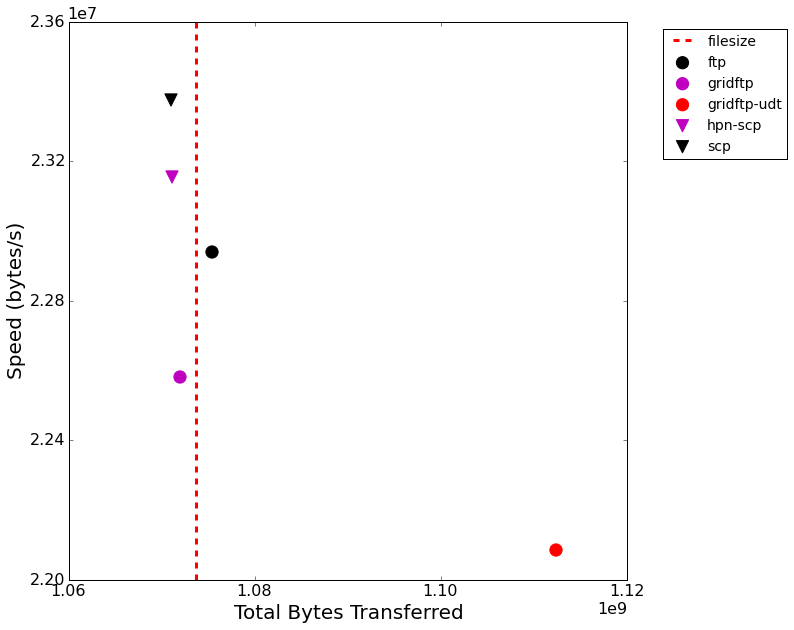
\includegraphics[width=\linewidth]{img/speed_bytes/1G.png}
	\caption{1 Gigabyte}
	\label{speed_bytes_1G}
	\end{subfigure}
	% \\
	\begin{subfigure}{.3\linewidth}
	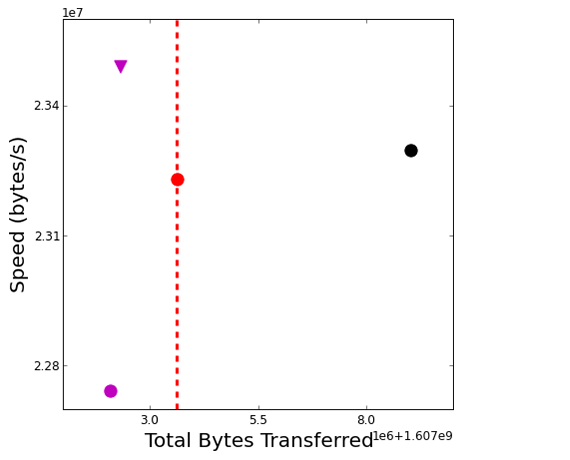
\includegraphics[width=\linewidth]{img/speed_bytes/1_5G.png}
	\caption{1.5 Gigabytes}
	\label{speed_bytes_1_5G}
	\end{subfigure}
	\begin{subfigure}{.3\linewidth}
	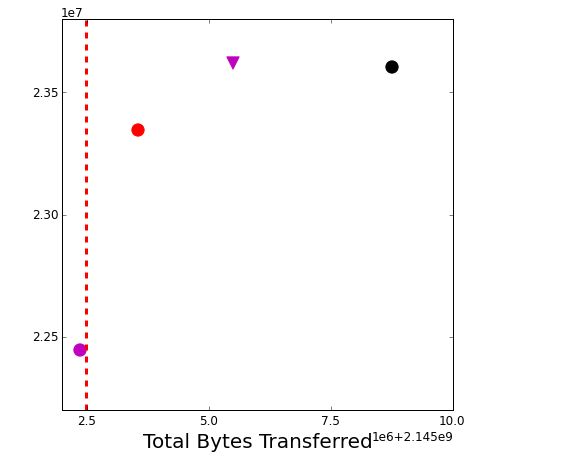
\includegraphics[width=\linewidth]{img/speed_bytes/2G.png}
	\caption{2 Gigabytes}
	\label{speed_bytes_2G}
	\end{subfigure}
	\begin{subfigure}{.3\linewidth}
	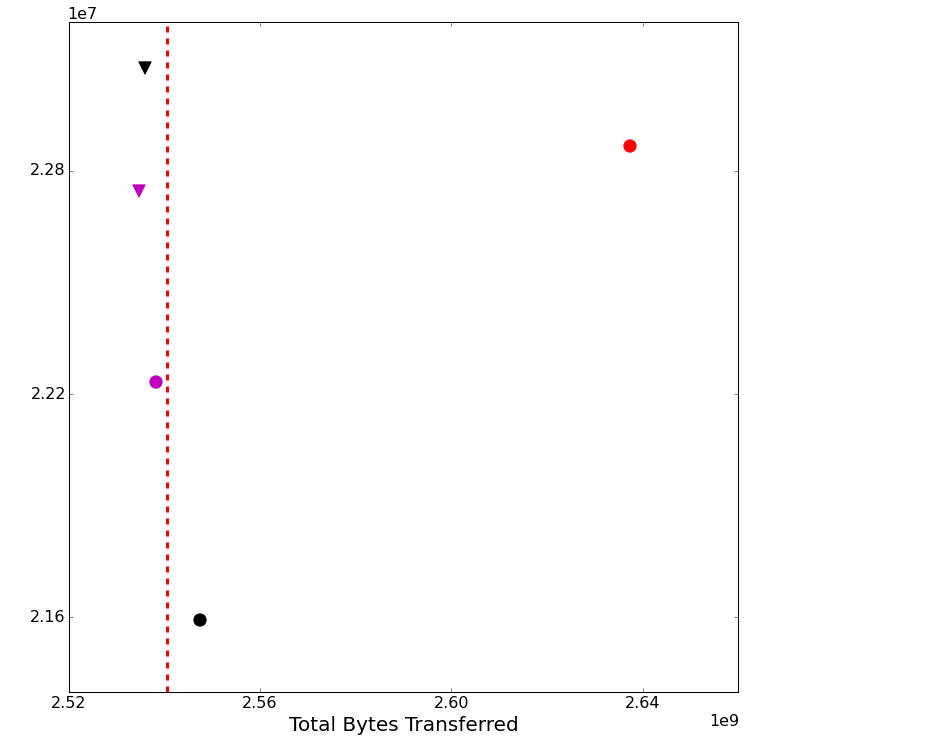
\includegraphics[width=\linewidth]{img/speed_bytes/2_4G.png}
	\caption{2.4 Gigabytes}
	\label{speed_bytes_2_4G}
	\end{subfigure}
\caption{Aggregated data per protocol. The dashed-red line represents the file size. Points to the left and right of the line are compressed/have overhead.}
\label{fig:aggregate}
\end{figure*}

Figure~\ref{fig:aggregate} is a comparison between all five protocols measuring the total speed, and total bytes. This is aggregated across all tests for each protocol. Note that the speed calculations only include downstream data, while the `transferred data' measures include data that is sent from the client back to the server via control channels etc. The dashed red line in each plot represents the size of the transferred file, and can be used for quick reference to see if a particular transfer protocol sends more or less data than the filesize on average. If the point lies to the right of the red line, the transfer has an overhead on average. If the point is on the left, the protocol has managed to send compressed data in an efficient way.

The corresponding numerical data (including upstream packets) can be seen in Table~\ref{tab:aggregate}.

\begin{figure}[h]
\centering
	\begin{subfigure}{.4\textwidth}
	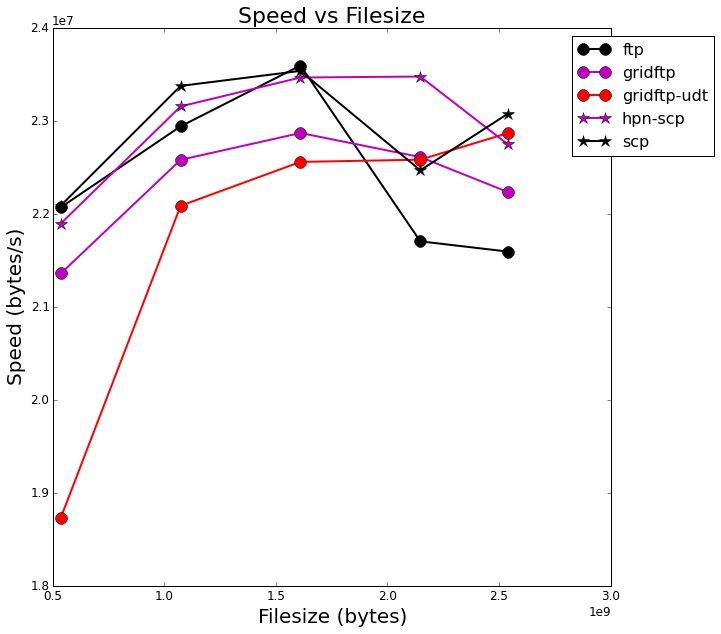
\includegraphics[width=\textwidth]{img/per_filesize/speed.png}
	\caption{Speed}
	\label{fig:per_fs_speed}
	\end{subfigure}
	\begin{subfigure}{.4\textwidth}
	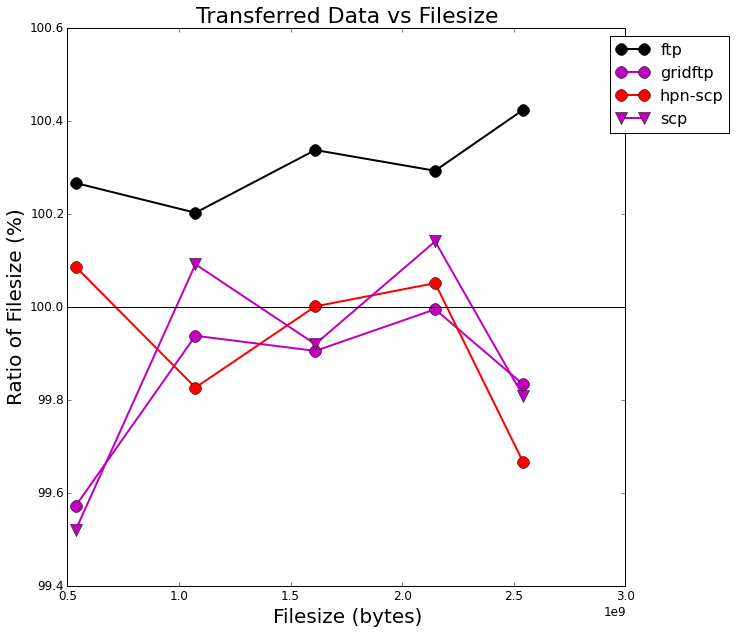
\includegraphics[width=\textwidth]{img/per_filesize/data.png}
	\caption{Data Efficiency}
	\label{fig:per_fs_data}
	\end{subfigure}
\caption{Metrics calculated per file size}
\label{fig:per_fs}
\end{figure}

This same data can be represented as a function of filesize. In this case, Figure~\ref{fig:per_fs_speed} compares the speed of each protocol for all tested file sizes. Surprisingly, the only protocols that are good consistently are SCP and HPN-SCP. GridFTP is consistently average, while FTP GridFTP-UDT change drastically with file size. 

It must be noted that the differences in speed are quite small at this scale (the graph is scaled to $10^6$).

Figure~\ref{fig:per_fs_data} shows the transferred data as a ratio of the file's size. A ratio of 100\% would mean that the total number of bytes transferred (both up and downsteam) is exactly the file size. Ratios larger and smaller than this are more and less data efficient respectively.

Here, one can see that GridFTP, HPN-SCP and SCP all achieve some level of optimization, as they sit between 99.5\% and 100\%. FTP sits close to, but just above this line between 100\% and 100.5\%. GridFTP-UDT is an outlier in this case, and clearly sends much more data than the TCP-based protocols.

One might assume that UDP transfers would use less data than TCP ones because UDP packets are not acknowledged by the host (requiring downstream data as well as upstream for each packet). This is not the case, because TCP acknowledgement packets are very small and tend not to make much of a difference. In fact, during some analysis, the downstream data was removed completely. The resulting plots were almost identical to the ones that included that data. The overhead can instead be explained by UDP's lack of redundancy, and it is rare (but not impossible) for data to be sent more than once.

In a practical sense, all 5 protocols save GridFTP-UDT have roughly the same efficiency, where both compression and overhead are less than 0.5\%. GridFTP-UDT uses slightly more data (less than 5\% overhead) which is not significant in most circumstances.

\section{Conclusions}
While transferring large datasets is not ideal, alternatives are not mature enough to remove the need completely. Cloud solutions are viable in some circumstances, but their shortcomings result in many situations where manually copying large files is unavoidable.

In these cases, it is only logical to make sure that the transfer is done in the fastest and most efficient way possible. An easily-deployable testbed has been created to test a specific connection and provide data which can be used to determine the most optimized solution.

This testbed was deployed on a LAN network, a conventional home internet connection, and a high-speed research and education network. The results from the SANReN connection between the Universities of Cape Town and the Western Cape were compiled and analysed. The traditional FTP and SCP were tested, as well as their newer counterparts, GridFTP and HPN-SCP.

Tests were run during lunch hours, and early hours of the morning. The data dumps from these tests were analysed using the testbed's supplementary Jupyter notebook. It was found that there was no significant difference between the speeds during peak and off hours. However, there were interesting artefacts in the few cases where the network was congested.

It was found that the TCP-based protocols achieved very similar speeds and data efficiency. GridFTP's `UDT' mode is built on UDP, and had a much higher overhead than the TCP protocols. The findings of Bresnahan et al.~\cite{bresnahan2009udt} were replicated, and GridFTP in UDT mode outperformed it's default mode for larger file sizes on this network.

Finally, it can be said that there were no significant improvements observed from the newer protocols. SCP and FTP both remained fast and efficient on the connection, where GridFTP and HPN-SCP were either mediocre, or changed with file size.

Of course, out of these four protocols, GridFTP remains the best choice for a fully configured data centre, as it can make use of striping and more complex authentication. However, if a researcher needs to copy a file now and then, SCP is still a solid choice, with the option of gaining some efficiency by applying the HPN patches with little effort.

In the future, it will be worthwhile to run these same tests on a network achieving over 1Gbit/s to see if the same results are yielded. This can be easily done by deploying the testbed described in this paper.

\section{Acknowledgements}
This project would not have been possible without access to virtual machines at both UCT and UWC. Mr. Peter van Heusden (South African Bioinformatics Institute) was extremely available during the project period, and kindly set up a VM in the SANBI DMZ. He also granted access to the Cisco switch which allowed rules for each protocol to be configured. Mr. Heine de Jager provided access to the UCT Science DMZ, and was very accommodating under strict security protocols. He was also extremely available, and helped fix multiple issues with the GridFTP setup and firewall rules.

\begin{table*}[t]
\centering
	\begin{tabular}{rlrrrrrr}
	\toprule
	File Size (bytes) &     Protocol &   Bytes Down &   Bytes Up &  Bytes Total &  Ratio (\%) &  Time (s) &  Speed (bytes/s) \\
	\midrule
	   5242880 &          ftp &    8413007.7 &   110014.3 &    8523022.0 &      162.6 &       1.4 &        9092596.7 \\
	           &      gridftp &    7412012.0 &  5270788.4 &   12682800.4 &      241.9 &       1.3 &        5560789.2 \\
	           &  gridftp-udt &    5543205.4 &     6239.1 &    5549444.5 &      105.8 &       2.7 &        2121498.5 \\
	           &      hpn-scp &    5095229.0 & 22532226.6 &   27627455.6 &      527.0 &       1.0 &        5339580.5 \\
	           &          scp &    4808391.8 &   104417.7 &    4912809.5 &       93.7 &       1.0 &        4907455.3 \\
	\midrule
	 536870912 &          ftp &  534084205.9 &  1298533.8 &  535382739.7 &       99.7 &      24.4 &       22069687.9 \\
	           &      gridftp &  535240945.3 &     4425.0 &  535245370.3 &       99.7 &      25.3 &       21358608.5 \\
	           &  gridftp-udt &  553768959.7 &   173186.2 &  553942145.9 &      103.2 &      30.2 &       18732210.9 \\
	           &      hpn-scp &  535401726.9 &   164294.4 &  535566021.3 &       99.8 &      24.7 &       21895264.8 \\
	           &          scp &  535381827.3 &   185875.7 &  535567702.9 &       99.8 &      24.4 &       22088599.5 \\
	\midrule
	1073741824 &          ftp & 1072881895.1 &  2558993.1 & 1075440888.1 &      100.2 &      47.1 &       22940550.1 \\
	           &      gridftp & 1071918333.8 &     4422.0 & 1071922755.8 &       99.8 &      47.6 &       22580395.8 \\
	           &  gridftp-udt & 1112012162.9 &   340049.3 & 1112352212.1 &      103.6 &      50.4 &       22086429.9 \\
	           &      hpn-scp & 1070826111.6 &   341411.1 & 1071167522.6 &       99.8 &      46.3 &       23154917.1 \\
	           &          scp & 1070596084.3 &   382239.0 & 1070978323.3 &       99.7 &      46.1 &       23375141.7 \\
	\midrule
	1610612736 &          ftp & 1609012156.9 &  3810770.9 & 1612822927.7 &      100.1 &      68.3 &       23594127.5 \\
	           &      gridftp & 1608155406.3 &     4423.1 & 1608159829.5 &       99.8 &      70.5 &       22868925.7 \\
	           &  gridftp-udt & 1668742869.2 &   507308.4 & 1669250177.6 &      103.6 &      74.0 &       22557996.6 \\
	           &      hpn-scp & 1608701999.0 &   513687.6 & 1609215686.6 &       99.9 &      68.7 &       23465480.1 \\
	           &          scp & 1608169009.5 &   581313.7 & 1608750323.2 &       99.9 &      68.4 &       23536710.8 \\
	\midrule
	2147479552 &          ftp & 2144495341.4 &  5166344.3 & 2149661685.7 &      100.1 &     100.0 &       21704026.4 \\
	           &      gridftp & 2145845215.4 &     4422.5 & 2145849637.9 &       99.9 &      95.0 &       22610027.5 \\
	           &  gridftp-udt & 2228159986.6 &   676775.8 & 2228836762.4 &      103.8 &      98.7 &       22581830.1 \\
	           &      hpn-scp & 2145264352.9 &   687628.8 & 2145951981.7 &       99.9 &      91.5 &       23476005.1 \\
	           &          scp & 2148226021.1 &   753291.0 & 2148979312.1 &      100.1 &      96.2 &       22467830.4 \\
	\midrule
	2540610608 &          ftp & 2541336324.7 &  6128837.9 & 2547465162.6 &      100.3 &     118.9 &       21593507.4 \\
	           &      gridftp & 2538172141.5 &     4412.9 & 2538176554.4 &       99.9 &     114.3 &       22233098.8 \\
	           &  gridftp-udt & 2636682223.1 &   799058.2 & 2637481281.3 &      103.8 &     115.3 &       22868390.6 \\
	           &      hpn-scp & 2533961524.4 &   806759.9 & 2534768284.3 &       99.8 &     111.9 &       22745305.3 \\
	           &          scp & 2535048746.9 &   908753.4 & 2535957500.3 &       99.8 &     110.2 &       23077735.8 \\
	\bottomrule
	\end{tabular}
\caption{Numerical data aggregated data per protocol}
\label{tab:aggregate}
\end{table*}

\bibliographystyle{abbrv}
\bibliography{ref}

\end{document}

